\chapter{Design \& Implementation}

This chapter will explore how the data set, and various machine learning models were created, using the decisions already discussed in Chapter \ref{ch:Requirements_Analysis}.

\section{Data Set Creation Process}

Taking into consideration all the data set decisions discussed in Section \ref{sec:Dataset_Decisions}, the data set creation process was split up into sequential steps.

\subsection{Combining Publicly Available Data Sets}

To create our data set, we started by combining the publicly available data sets provided by \citet{Singh2020, Zhang2008, Gao2017, Zhang2008}. All columns were removed except the ones with the SMILES notation, drug or compound name, experimental logBB value and blood-brain barrier permeability. We felt that this was the most appropriate strategy as all data sets used a vast array of chemical descriptors from different sources. Furthermore, this would allow us to retain the most essential information that we could then build upon.

Each academic paper's Digital Object Identifier (DOI) was provided as the source for compounds and drugs. When it was not available, either a link to \citet{PubMed} or \citet{PubMed_Central} was provided as the source.

It should also be noted that when the experimental logBB was available, BBB permeability was recalculated using the thresholds suggested by \citet{Li2005}:

$$ BBB+ \text{ if } LogBB >= -1 $$
$$ BBB- \text{ if } LogBB < -1  $$

Given that the vast majority of the data set was created using the process discussed above, its quality is as good or bad as those data sets it has built upon.

\subsection{Automated Google Searches}

In an effort to expand our data set, we initially decided to perform some basic text mining using automated google searches, using \citet{Google_Package}, querying about specific drugs and compounds not present in our data set and their relation to the blood-brain barrier.

Our strategy was to gather the first 10 URLs returned from our google search and their HTML contents, and then using regular expressions, try to find matches for our query, hopefully leading to an apparent relationship between our specific drug or compound and the blood-brain barrier. These matches and their associated URLs were then loaded onto excel files and manually verified or rejected. Unfortunately, this strategy was proven to be too targeted and ineffective, returning completely irrelevant results most of the time.

Learning from our experience and discovering a class imbalance heavily tilting towards BBB+ drugs and compounds in our data set, we decided to broaden our search to try and reduce this imbalance, querying about drugs and compounds unable to cross the blood-brain barrier.

We followed the same process as before, but this time collecting as many URLs as we could before getting a "429: Too many requests error" and using multiple variations of queries and regular expressions, as showcased in Listing \ref{lst:Queries}. Unfortunately, this strategy was also proven ineffective, returning results from online forums and sites clearly having nothing to do with peer-reviewed medical or chemical information. 
Even though we had collected some usable results from these strategies, we decided not to use them as someone could argue that they are incredibly unreliable and noisy. Discussion on how to overcome these shortcomings led us to the discovery of the medical APIs explored in the next section.

\begin{lstlisting}[language=python, label={lst:Queries}, caption={A small sample of the list of queries and regular expressions used in an effort to expand our data set using Google Searches.}]
    queries_and_regular_expressions = [

    ["\"not able to cross the blood brain barrier\"", ".*was not able to cross the blood.brain barrier.*"],
    ["\"not able to cross the bbb\"", ".*was not able to cross the bbb.*"],
    ["\"not able to penetrate the blood brain barrier\"", ".*was not able to penetrate the blood.brain barrier.*"],
    ["\"not able to penetrate the bbb\"", ".*was not able to not penetrate the bbb.*"],
    ["\"not able to pass through the blood brain barrier\"", ".*was not able to pass through the blood.brain barrier.*"],
    ["\"not able to path through the bbb\"", ".*was not able tp pass through the bbb.*"],
    ["\"not able to get through the blood brain barrier\"", ".*was not able to get through the blood.brain barrier.*"],
    ["\"not able to get through the bbb\"", ".*was not able to get through the bbb.*"]
    
    ]
\end{lstlisting}

\subsection{Medical APIs}

\citet{PubMedAPI} was used to get abstracts from \citet{PubMed} and academic papers from \citet{PubMed_Central} that matched multiple queries about drugs and compounds unable to penetrate the blood-brain barrier.

The various paragraphs of the abstracts and academic papers were extracted using XML parsing, and then, just as before, regular expressions were used to find matches based on our query. Finally, the matches were again loaded into excel files and manually verified.

\citet{PubMed} searches produced 15 usable drugs and compounds, 14 being BBB- and 1 surprisingly being BBB+, from 35 matches.

\citet{PubMed_Central} searches produced 91 usable drugs and compounds, with all being BBB-, from 361 matches.

\citet{SpringerAPI} was used to get abstracts, articles and journals and then the same process was used just as in the case above.

Springer Meta V2 searches allowed us to access the abstracts of articles and journals not open to the public and produced 42 usable drugs and compounds, with 41 being BBB- and 1 being BBB+, from 108 matches.

Springer Open access searches allowed us to access the publicly available full-text content of articles and journals and produced 109 usable drugs and compounds, with 106 being BBB- and 3 being BBB+, from 491 matches.

As mentioned above, the matches returned by the API searches had to be manually verified, and it should be mentioned that any human validated data is bound to have at least a few errors.

\subsection{Retrieving Chemical Descriptors, Side Effects \& Indications}

Once we had gathered all the drugs and compounds from the publicly available data sets and our API searches, \citet{PubChemAPI} was used to retrieve the chemical descriptors, already mentioned in Subsection \ref{subsec:Chemical_Descriptors}, as well as some other helpful information such as the PubChem CID, the unique identifier for each compound in the \citet{PubChem} database, the synonyms associated for each compound and its most common name, which was essentially the first synonym available. Even though the name of the compound was supplied in most of the cases by the data sets we had combined, we felt that it would make things easier down the road, and for anyone in the future that might utilise this work, if we used replaced it with the one in the PubChem database. 

We mainly used the SMILES notation of each drug or compound to search the PubChem database for a match to accomplish this task. If the SMILES notation was unavailable, we used the drug or compound name to search for a match. Naturally, we discovered that using the drug or compound name was less effective in getting a match from the database than the SMILES format, as the latter is unique for each drug or compound, whereas multiple drugs or compounds can use the same name, which can lead to confusion.

It should also be noted that some drugs and compounds do not have a name or any synonyms associated with them.

Once the synonyms were retrieved for a specific drug or compound, they were looked up in the \citet{SIDER} database. If a synonym was found in the SIDER database, we then retrieved the SIDER CID and the associated side effects and indications. 

SIDER offered two types of labels for side effects and indications, Lowest Level Terms (LLTs), taken directly from the official description of drugs, and Preferred Terms (PTs), which simplify multiple LLTs. We decided to use the PT side effects and indications since they condensed multiple LLTs.

\subsection{Final Adjustments}

Duplicates, drugs and compounds that could not be discovered and those without all chemical descriptors available were removed. This process decreased the size of the data set from 3748 drugs and compounds to 2396, with 1751 being BBB+ and 645 being BBB-. The data set was then finally sorted by drug name.

Table \ref{tbl:Dataset} showcases the first 10 rows of the final version of the data set.

\begin{table}[ht!]
  \caption{The first 10 rows of our finalised data set.}
  \label{tbl:Dataset}
  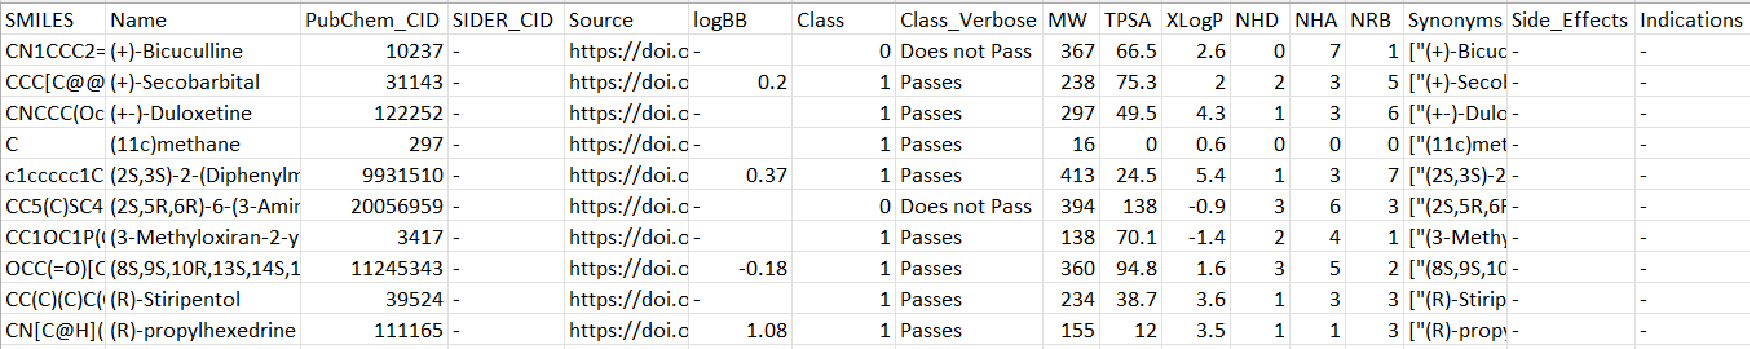
\includegraphics[width=1.0\linewidth]{images/Dataset.pdf}
\end{table}

\section{Model Training \& Testing Process}

Our training and testing process was straightforward and used consistently for both classification and regression models.

We would first create a pipeline \citep{Pipeline} containing a model and a standard scaler \citep{StandardScaler}. Pipelines simplify our workflow by stacking several pre-processing steps that are applied to our data before they are passed to a chosen model as features. In our case, we are just using a standard scaler as a pre-processing step that normalises our features by "removing the mean and scaling to unit variance".

We would then pass this pipeline to GridSearch \citep{GridSearch} as the estimator along with the specific model parameters we wanted to tune, the metrics we wanted to be returned, the metric we wanted to optimise for and the number of cross-validation folds. This process is showcased by Figure \ref{fig:Optimisation} to make things clearer.

All models were optimised using a 10-fold cross-validation GridSearch except in the case of the dummy classifier, dummy regressor and linear regression models.

Once optimised, the models were then tested for robustness, using permutation testing as already discussed in \ref{subsec:Robustness}, and used to make predictions on their respective test set.

\begin{figure}[htb]
    \centering
    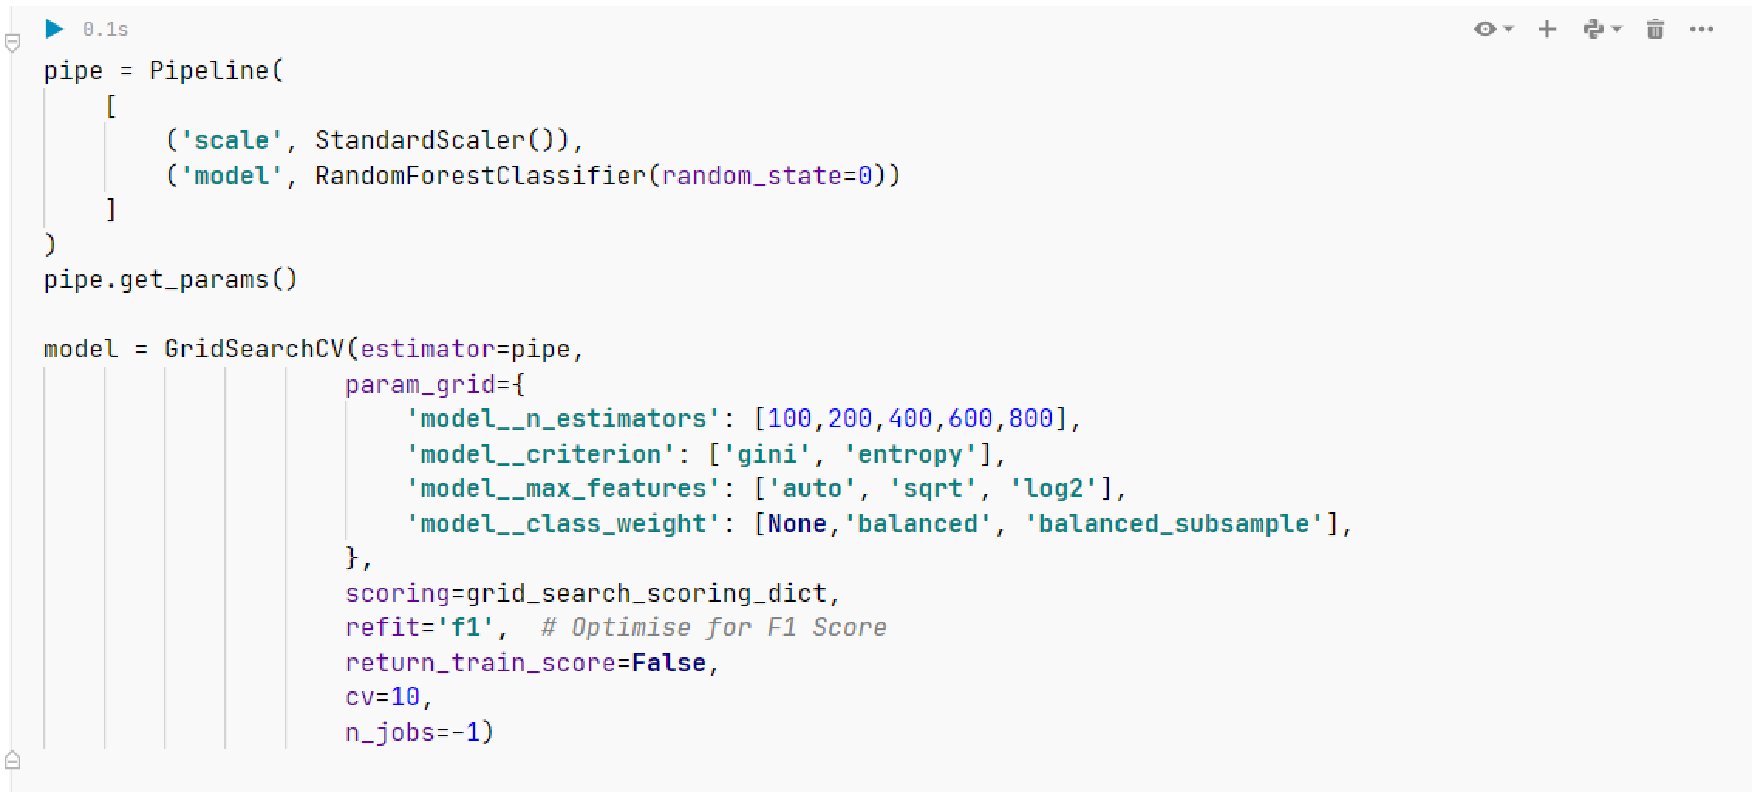
\includegraphics[width=1.0\linewidth]{images/Optimisation.pdf}    
    \caption{The optimisation process used for the majority of our models, showcased with a Random Forest Classifier.}

    \label{fig:Optimisation} 
\end{figure}

\subsection{Classification Models}
\label{subsec:Classification_Models}

Classification models were split up into two categories, one using just the chemical descriptors as features and the other using the chemical descriptors and a selection of one-hot encoded side effects and indications as features.

A selection was used instead of every single side effect and indication supplied by \citet{SIDER} to not only improve the training times of our models but to also potentially discover which side effects and indications play the most critical role in deciding blood-brain barrier permeability. To achieve this, we decided to use scikit-learn's recursive feature elimination with cross-validation (RFECV) function \citep{RFECV} which does exactly what it suggests, with a random forest classifier, optimising for F1 score, and a 10-fold cross-validation. As a result, RFECV managed to reduce our features from 4353 to 217, keeping all 6 chemical descriptors, 196 of the side effects and 15 of the indications.

We decided to split our classification models into two separate categories because we were interested in discovering whether the addition of side effects and indications to the chemical descriptors improved their predictive performance. Therefore, we needed a common holdout test set to achieve this.

This holdout test set was a 20\%  stratified split of the 345 drugs and compounds that had chemical descriptors, side effects and indications available (199 BBB+, 146 BBB-), produced with scikit-learn's Train Test Split function \citep{TrainTestSplit}. 

The training sets for both categories excluded the drugs and compounds present in the test set, with the first category making use of the whole data set, while the second one used the subset of drugs and compounds having chemical descriptors, side effects and indications available.

Finally, the classification models we decided to train for both categories were:
\begin{itemize}
    \item 
    Dummy Classifier
    \item 
    Logistic Regression
    \item 
    Support Vector Classifier
    \item 
    K-Nearest Neighbour Classifier
    \item 
    Random Forest Classifier
    \item 
    Decision Tree Classifier
    \item 
    Stochastic Gradient Descent Classifier
\end{itemize}

\subsection{Regression Models}

Regression models were solely trained using chemical descriptors as there were not enough drugs and compounds with logBB values available and chemical descriptors, side effects and indications to split them into two categories just as it was done in the case of the classification models.

The training and test sets were again produced using scikit-learn's Train Test Split function \citep{TrainTestSplit}. The holdout test set was a 20\% stratified split of the 401 drugs and compounds that had logBB values available (360 BBB+, 41 BBB-). The remaining 80\% was used as the training set.

Finally the regression models we decided to train were:
\begin{itemize}
    \item 
    Dummy Regressor
    \item 
    Linear Regression
    \item 
    Support Vector Regression
    \item 
    K-Nearest Neighbour Regressor
    \item 
    Random Forest Regressor
    \item 
    Decision Tree Regressor
    \item 
    Stochastic Gradient Descent Regressor
\end{itemize}


\section{Streamlit Web App}

The web app was created in the final weeks of the project to present a synopsis of our work and primarily showcase our models and to allow users to make predictions with them. A strong emphasis was also placed on model interpretability, helping users understand what led to a specific prediction by a model, which was already briefly discussed in Subsection \ref{subsec:Interpretability}. However, it should be noted that these interpretability tools are not available for all models.

Figure \ref{fig:Streamlit} showcases a prediction made by our trained Random Forest Classifier using our web application, and the interpretability tools, which a user can use to try and understand the model's prediction.

\href{https://share.streamlit.io/georgeiniatis/blood_brain_barrier_drug_prediction/main/Streamlit_App/app.py}{\textbf{You can access the web application using this link}}

\begin{figure}[htb]
    \centering
    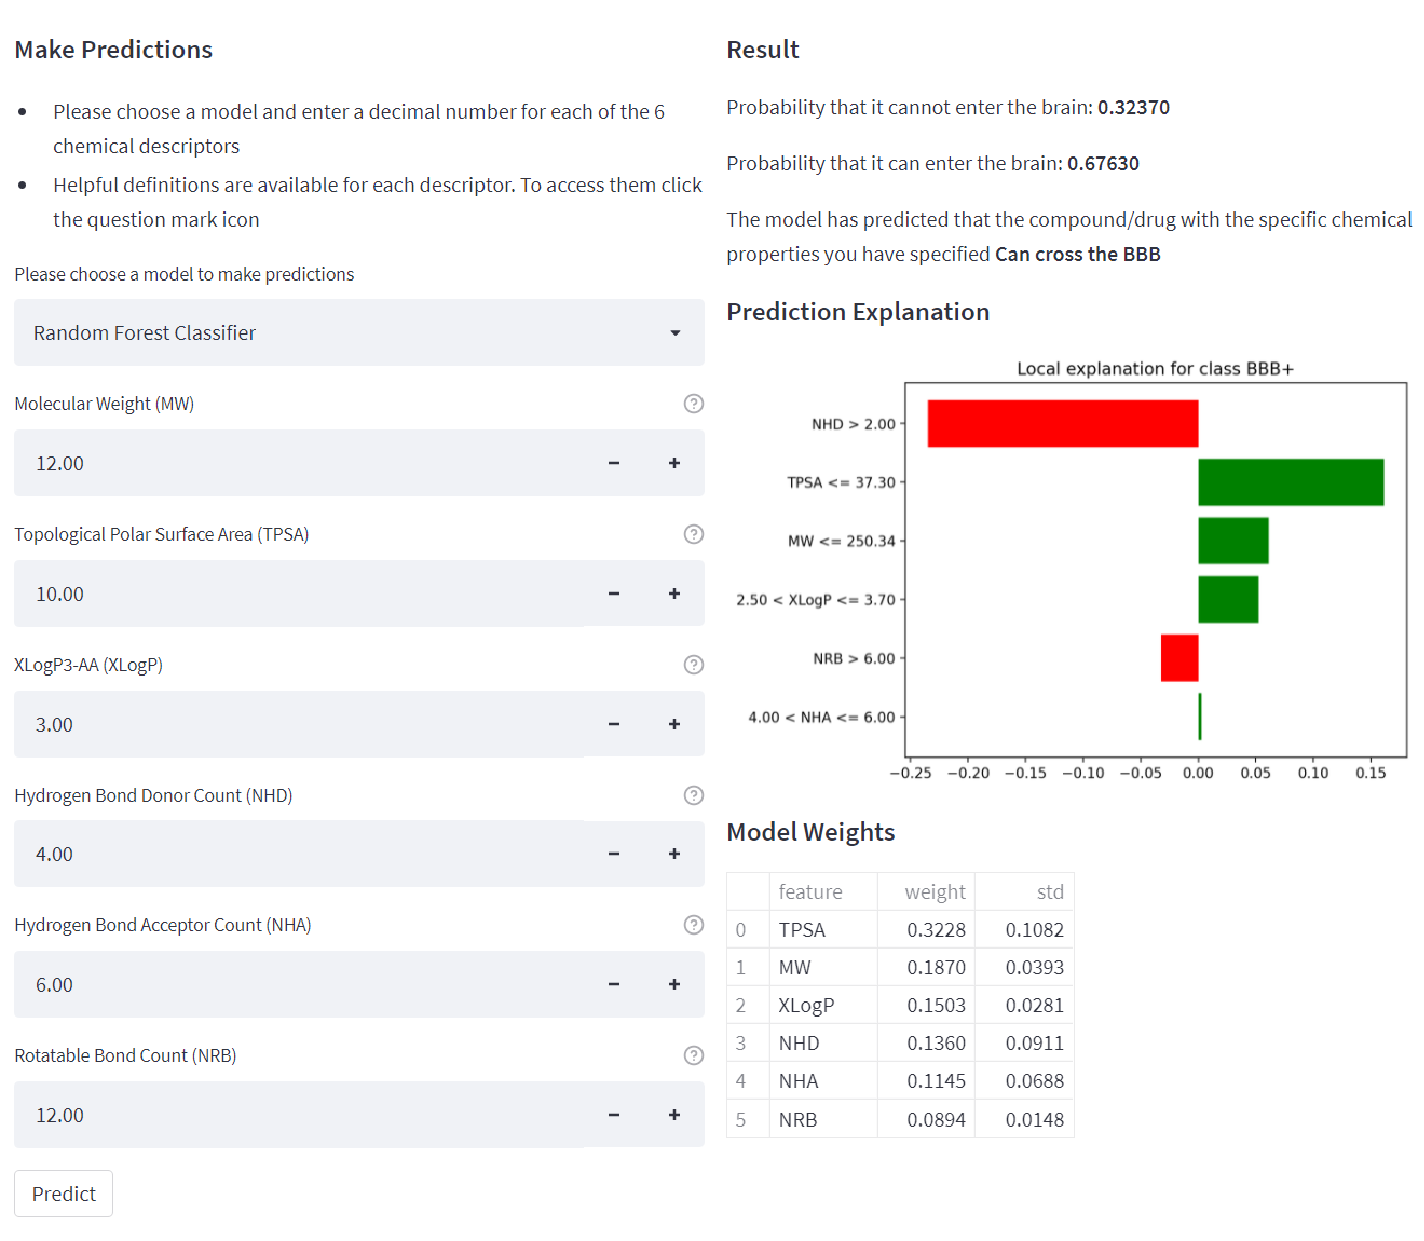
\includegraphics[width=0.8\linewidth]{images/Streamlit.pdf}    
    \caption{Our trained Random Forest Classifier used to make a prediction in our Streamlit Web App.}

    \label{fig:Streamlit} 
\end{figure}


 


